\chapter{Open Quantum Systems}
\label{Chapter1}
\epigraph{The motivation for studying open systems is that all realistic systems are open.}{\textit{John Preskill}}

% Define some commands to keep the formatting separated from the content 
\newcommand{\keyword}[1]{\textbf{#1}}
\newcommand{\tabhead}[1]{\textbf{#1}}
\newcommand{\code}[1]{\texttt{#1}}
\newcommand{\file}[1]{\texttt{\bfseries#1}}
\newcommand{\option}[1]{\texttt{\itshape#1}}

%----------------------------------------------------------------------------------------
The world we live in is constituted by parts that communicate with each other and exchange information. The difficulty of describing it, lies in the complexity of the interactions between those parts. To overcome this problem, simplifications and easier mathematical representations have been developed: in the following we will see some of them.

However, before getting into the topic, it is worth to discuss \emph{why} the field of open quantum systems have become of great physical interest.

One of the main goals in scientific research is coming up to quantum simulation; this is due to the fact that in several physical fields there are mechanisms that cannot be simulated by classical computers: the essential aim is using a controlled quantum device to investigate another quantum system. Experiments have shown that superconducting circuits are able to manipulate and measure at the level of a few qubits and microwave photons, as a quantum simulator~\cite{Nat.Phys2012}. They can be treated as open systems because of the loss of photons, coupled to the feeding in additional photons through continuous external driving. Moreover, they are greatly flexible, because of their nanofabricated nature and almost every parameter involved is widely tunable. In~\cite{PhysRevX.7.011016}, it has been demonstrated that QED cavity lattices act as a controllable platform guiding understanding of non-equilibrium physics. 

\begin{figure}
    \centering
    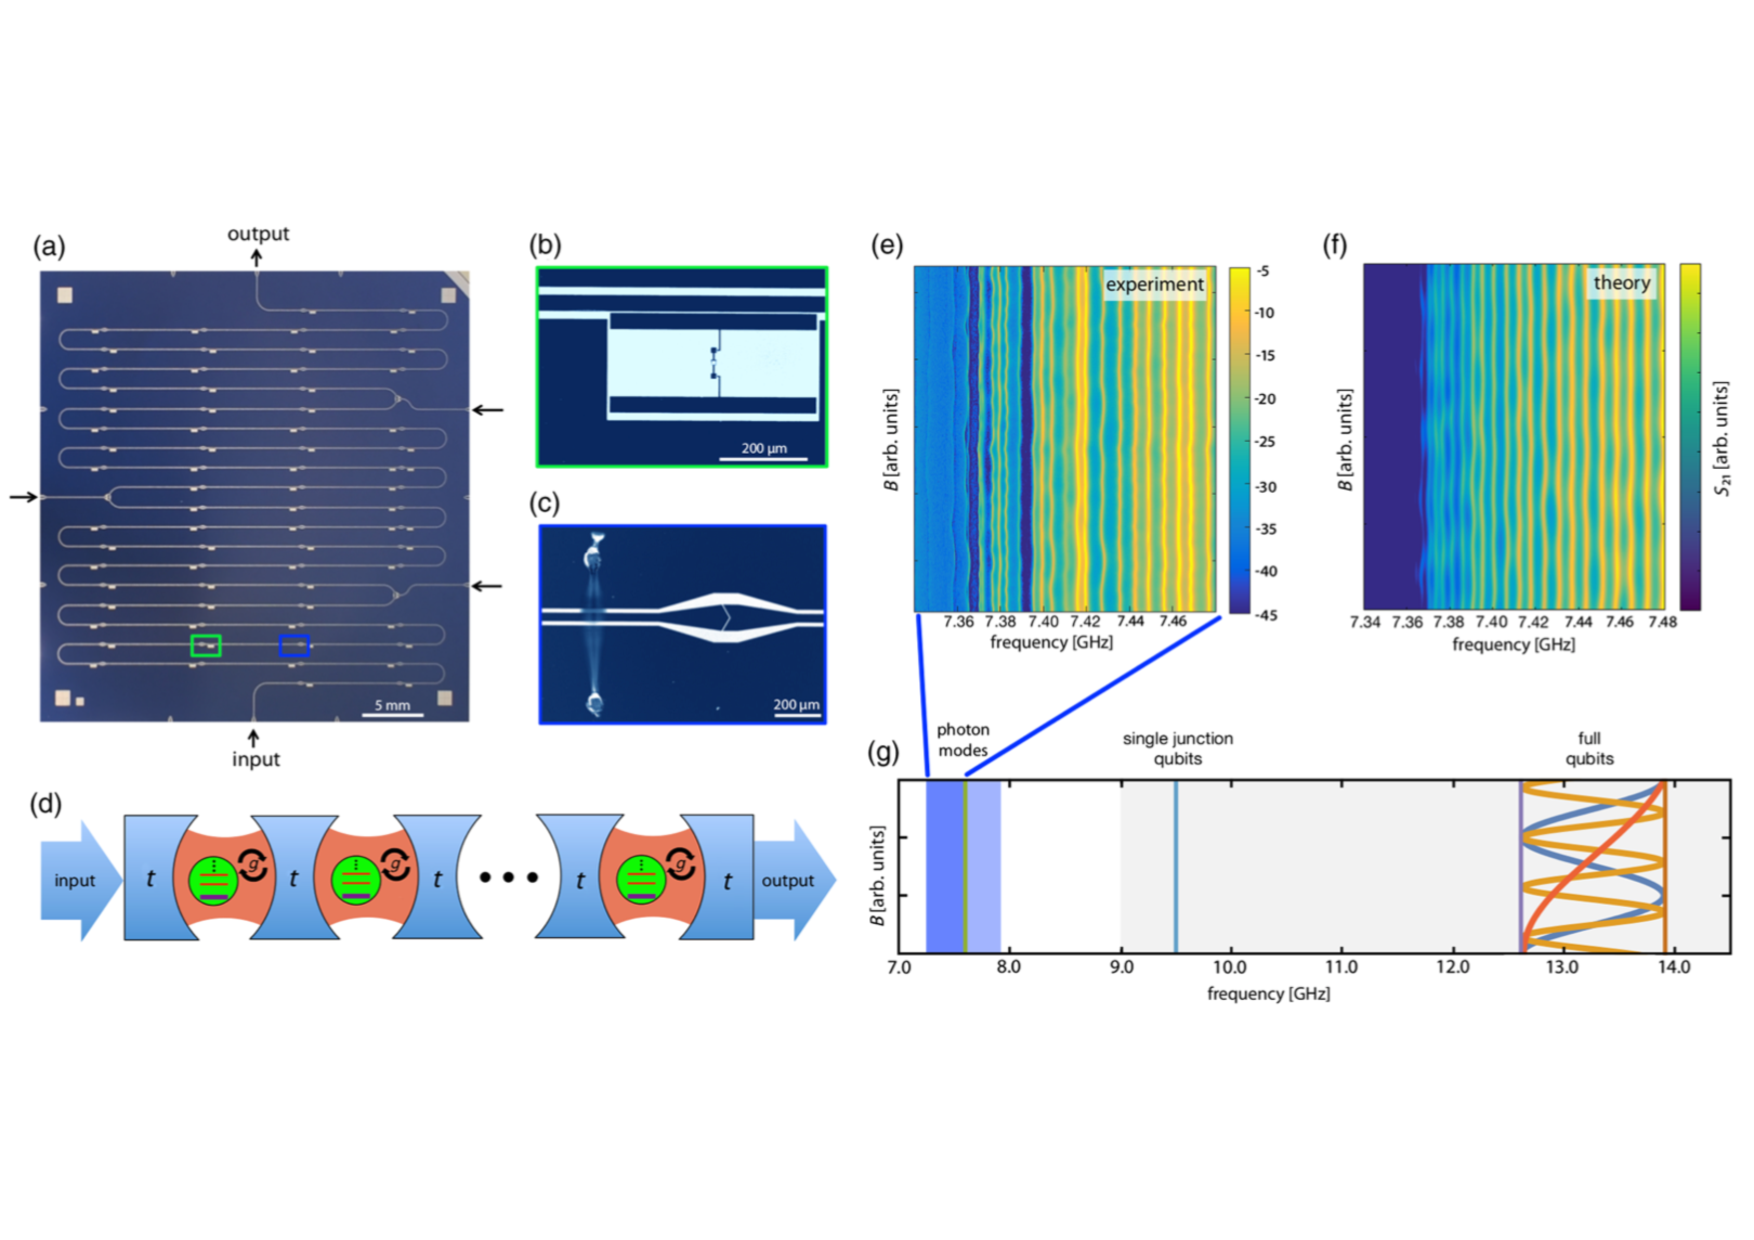
\includegraphics[scale=0.5]{Figures/PhysRevX_image_7011016.pdf}
    \caption{Caption}
    \label{fig:my_label}
\end{figure}

Another approach to quantum simulation has been developed by means of ultracold atoms, useful in the study of strongly correlated ground states~\cite{nphys1073}. 

As explained in~\cite{Noh_2016}, an important contribution has been done with the introduction of coupled resonator arrays (CRA)\dots

This chapter has the purpose of giving a recap of the most useful characteristics of open quantum systems, in the perspective of studying an open many-body system and, as stated before, a 1D spin chain, in particular. First of all, in section~\ref{cl_open_qs} we will specify the difference between closed and open systems and we will derive the density matrix formalism; then, in section~\ref{appr_dynam_oqs} we will gather the master equation useful for describing the dynamics of open quantum systems; finally, in section~\ref{many_body_oqs} we will see some properties of open many-body quantum systems, that we will use effectively in the original part of the present work.

\section{Closed and Open Quantum Systems}
\label{cl_open_qs}
Before we explore the field of open quantum systems, we now observe what the differences between a closed and an open quantum system are and why different approaches are required to treat these two distinct kinds of system. First of all, let us define a \emph{closed} system as a physical system which does not exchange any information with its surroundings. On the contrary, an \emph{open} system is a physical system that interacts with the environment in which it is. 

In this section, we will briefly look at the different approaches in the study of the dynamics in closed and open quantum systems. 

\subsection{Pure and mixed states: the density matrix formalism}
First of all, it is useful consider another formalism in addition to that used normally for handling pure states, i.e. states that can be described by a single wave function. We now introduce the \emph{density matrix} formalism for managing the so-called mixed states, although - as we will see - it can be used also for pure states.

Quantum systems prepared in such a way that their state vector being obtained performing a \emph{maximal measurement}, in the sense that the maximum possible information has been acquired (all values of a complete set of commuting observables have been ascertained), are in a pure state. 

Quantum systems for which the maximum possible information is not available, are said to be in mixed state and are called \emph{statistical mixtures}.

Let us consider a system consisting of an ensemble of N sub-systems $\alpha = 1, 2, \dots , N$. We suppose that every sub-system is in a pure state $\ket{\psi_\alpha}$. Then, we choose a complete set of basis vectors $\ket{n}$, such that $\sum_n \ket{n}\bra{n} = \mathds{1}$. Let us expand the pure states in the basis $\{\ket{n}\}$:
\begin{equation*}
    \ket{\psi_\alpha} = \sum_n c_n^{(\alpha)}\ket{n},
\end{equation*}
where the coefficients $c_n^{(\alpha)}$ are such that
\begin{equation*}
    \sum_n |c_n^{(\alpha)}|^2 = 1.
\end{equation*}
Now let us consider an observable represented by an operator $A$; its expectation value in the pure state $\psi_\alpha$ is:
\begin{align}
    \braket{A}_\alpha &= \bra{\psi_\alpha}A\ket{\psi_\alpha} \\
                      \label{braket_A}
                      &= \sum_n \sum_{n'} c_{n'}^{(\alpha)*} c_n^{(\alpha)} \bra{n'}A\ket{n} \\
                      &= \sum_n \sum_{n'} \braket{n|\psi_\alpha}\braket{\psi_\alpha|n'} \bra{n'}A\ket{n}.
\end{align}
The average value of A over the ensemble is
\begin{equation}
\label{stat_averageA}
    \braket{A} = \sum_{\alpha = 1}^N w_\alpha \langle A \rangle_\alpha,
\end{equation}
where the coefficients $w_\alpha$ are the statistical weight of the pure states $\ket{\psi_\alpha}$, i.e. the probability of finding the system in this state. 
So the $w_\alpha$ are such that
\begin{equation}
\label{charact_weights}
    0 \leq w_\alpha \leq 1
\end{equation}
and 
\begin{equation*}
    \sum_{\alpha=1}^N w_\alpha = 1.
\end{equation*}
Using the result~\ref{braket_A} in the~\ref{stat_averageA}, we obtain:
\begin{align}
    \braket{A} &= \sum_{\alpha = 1}^N \sum_n \sum_{n'} w_\alpha c_{n'}^{(\alpha)*} c_n^{(\alpha)} \bra{n'}A\ket{n} \\
                \label{total_stat_average}
               &= \sum_{\alpha = 1}^N \sum_n \sum_{n'} \braket{n|\psi_\alpha}w_\alpha \braket{\psi_\alpha|n'} \bra{n'}A\ket{n}.
\end{align}
We now introduce the \emph{density operator}
\begin{equation}
    \rho = \sum_{\alpha = 1}^N \ket{\psi_\alpha} w_\alpha \bra{\psi_\alpha},
\end{equation}
whose representation in the basis $\{n\}$ gives us the density matrix:
\begin{equation}
    \rho_{nn'} = \bra{n}\rho\ket{n'} = \sum_{\alpha = 1}^N w_\alpha c_{n'}^{(\alpha)*} c_n^{(\alpha)}.
\end{equation}
So, returning to the~\ref{total_stat_average} in the definition of the density matrix, we observe that:
\begin{equation*}
    \braket{A} = \sum_n \sum_{n'} \bra{n}\rho\ket{n'}\bra{n'}A\ket{n} = \Tr({\rho A}).
\end{equation*}
It is worth stressing the fact that the knowledge of the density matrix enables us to obtain the ensemble average of A.

Anyway, this leads us to the first of the three fundamental characteristics of the density matrix, that is:
\begin{equation}
    \Tr(\rho) = 1,
\end{equation}
that is true if we make the assumption that the $\ket{\psi_\alpha}$ are normalized to unity. If they are not, then the ensemble average of A is given by
\begin{equation}
    \braket{A} = \frac{\Tr(\rho A)}{\Tr(\rho)}.
\end{equation}
The second characteristic of the density matrix is that it is Hermitian, namely
\begin{equation}
    \bra{n}\rho\ket{n'} = \bra{n'}\rho\ket{n}^*.
\end{equation}
The third characteristic arises from the observation of the diagonal elements of $\rho$:
\begin{equation}
    \rho_{nn} = \bra{n}\rho\ket{n} = \sum_{\alpha = 1}^N w_\alpha |c_{n}^{(\alpha)}|^2,
\end{equation}
which tells us, with the~\ref{charact_weights}, that
\begin{equation}
    \rho_{nn} \geq 0,
\end{equation}
i.e. $\rho$ is a positive semi-definite matrix.
It is worth stress the physical interpretation of the diagonal elements; $w_\alpha$ is the probability of finding the system in the pure state $\psi_\alpha$, while $|c_{n}^{(\alpha)}|^2$ is the probability of finding $\psi_\alpha$ in the state $\ket{n}$. So, $\rho_{nn}$ gives the probability of finding a member of the ensemble in the state $\ket{n}$.

\subsection{Closed Quantum Systems}
\label{closed_systems}
Quantum mechanics establishes that the time evolution of a state vector $\ket{\psi(t)}$ is predicted by the Schrödinger equation:
\begin{equation}
\label{eqn:schrod_eq}
    i\frac{d}{dt}\ket{\psi(t)} = H(t)\ket{\psi(t)},
\end{equation}
where $H(t)$ is the Hamiltonian of the closed system and Planck's constant $\hbar$ has been set equal to 1.
The solution of this equation can be written in terms of the unitary time-evolution operator $U(t, t_0)$:
\begin{equation}
\label{eqn:schrod_u}
    \ket{\psi(t)} = U(t, t_0)\ket{\psi(t_0)},
\end{equation}
where $t_0 < t$. If we substitute the equation~\ref{eqn:schrod_u} into the~\ref{eqn:schrod_eq}, we obtain:
\begin{equation}
    i\frac{d}{dt}U(t, t_0) = H(t)U(t, t_0),
\end{equation}
subject to the initial condition
\begin{equation}
    U(t_0, t_0) = \mathds{1}.
\end{equation}
We can write the dynamics of a closed system using the density matrix formalism seen in the previous section. In order to do this, let us assume that at a initial time $t_0$ the state of the system is characterized by the density matrix
\begin{equation*}
    \rho(t_0) = \sum_{\alpha = 1}^N w_\alpha \ket{\psi_\alpha(t_0)} \bra{\psi_\alpha(t_0)},
\end{equation*}
that at a time $t$ evolves in this way:
\begin{equation*}
    \rho(t) = \sum_{\alpha = 1}^N w_\alpha U(t,t_0)\ket{\psi_\alpha(t_0)} \bra{\psi_\alpha(t_0)}U(t,t_0)^\dagger,
\end{equation*}
that is
\begin{equation*}
     \rho(t) = U(t,t_0) \rho(t_0) U(t,t_0)^\dagger.
\end{equation*}
Differentiating with respect to time the last equation we have
\begin{equation}
\label{eqn:motion_closed_dm}
    \frac{d}{dt}\rho(t) = -i[H(t), \rho(t)]
\end{equation}
i.e. an equation of motion for the density matrix, often called the \emph{Liouville-von Neumann equation}.


\subsection{Open Quantum Systems}
Now we can go into a more specific definition of open quantum systems. It can be defined as a system $S$ coupled with another quantum system $E$, called the \emph{environment}. Usually, the total system $S+E$ is treated as a closed system, so it follows Hamiltonian dynamics. The interactions between the two sub-systems cause an evolution in the state of the open system $S$, which can no longer be represented by unitary, Hamiltonian dynamics. Following the definitions given in~\cite{pet_breuer:open_quantum}, an environment with an infinite number of degrees of freedom such that the frequencies of the modes form a continuum, is called \emph{reservoir}. Also, when the reservoir is in thermal equilibrium state, is called \emph{bath}.

Let us call $\mathcal{H}_S$ and $\mathcal{H}_E$ the Hilbert spaces of the system and the environment, respectively. The Hilbert space of the combined system is given by the tensor product $\mathcal{H}_{S+E} = \mathcal{H}_S \otimes \mathcal{H}_E$. So, the total Hamiltonian can be written in this way:
\begin{equation}
    H(t) = H_S \otimes \mathds{1}_E + \mathds{1}_S \otimes H_E + H_I(t),
\end{equation}
where $H_S$ and $H_E$ are the free Hamiltonians of the system and the environment, respectively, and $H_I(t)$ is the Hamiltonian describing the interactions between $S$ and $E$.

At this point, we must find a relation between the density matrix $\rho \in \mathcal{H}$ and $\rho_S \in \mathcal{H}_S$; it is given by the partial trace over the environment $B$\footnote{A proof of this statement is given, e.g., by ref.~\cite{nielsen_chuang}.}:
\begin{equation}
    \rho_S = \Tr_E(\rho).
\end{equation}
This helps us in the study of the dynamics of the so-called \emph{reduced} density matrix $\rho_S$. Indeed, we can write:
\begin{equation}
    \rho_S(t) = \Tr_E\{\rho(t)\};
\end{equation}
observing that we assumed the total system to be \emph{closed}, it evolves unitarily so we have:
\begin{equation}
    \rho_S(t) = \Tr_B\{U(t, t_0)\rho(t_0)U(t, t_0)^\dagger\},
\end{equation}
where $U(t, t_0)$ is the time-evolution operator of the combined system $S+E$. So we can use the equation of motion~\ref{eqn:motion_closed_dm} and trace over the degrees of freedom of the environment, in order to obtain the equation of motion for the $\rho_S(t)$:
\begin{equation}
\label{eqn:motion_open}
    \frac{d}{dt}\rho_S(t) = -i \Tr_B[H(t), \rho(t)].
\end{equation}


%%%%%%%%%%%%%%%%%%%%%%%%%%%%%%%%%%%%%%%%%%%%
%%%%%%%%%%%%%%%%%%%%%%%%%%%%%%%%%%%%%%%%%%%%
\section{Approximate Dynamics of Open Quantum Systems}
\label{appr_dynam_oqs}
Solving exactly the equation~\ref{eqn:motion_open} is rather difficult, because of the fact that the environment may represent a reservoir consisting of infinitely many degrees of freedom, or its modes may be neither known nor controllable, for example. The following will derive a simpler description of the dynamics of an open quantum system. 

\subsection{Quantum Dynamical Semigroups}
For reasons that will be clear later, let us rewrite the equation~\ref{eqn:motion_open} as a \emph{dynamical map} acting on $\mathcal{H}_S$ that connect the states of the system $S$ from time $t_0$ to time $t_1$, that is:
\begin{equation}
    \matcal{\varepsilon}_{(t_1, t_0)}: \quad \rho_S(t_0) \mapsto \rho_S(t_1).
\end{equation}
In order to obtain the way in which this map acts on the states, we consider a system consisting in two sub-systems $S+E$, that are uncorrelated\footnote{Initial correlations between environment and the open system play significant role in the dynamics of open systems~\cite{PhysRevA.64.062106}.} at the initial time $t=0$, so that 
\begin{equation}
    \rho(0) = \rho_S(0) \otimes \rho_E(0),
\end{equation}
where $\rho_S(0)$ is the initial state of the system $S$ and $\rho_E(0)$ represents the state of the environment at time $t=0$. The evolution of the system $S$ from the time $t=0$ to the time $t>0$ is governed by the map, in this way:
\begin{equation}
\label{dynam_map}
    \rho_S(0) \mapsto \rho_S(t) = \matcal{\varepsilon}(t)\rho_S(0) \equiv \Tr_E \{U(t, 0)[\rho_S(0) \otimes \rho_E(0)] U^\dagger(t,0)\}.
\end{equation}
Using the spectral decomposition of the density matrix $\rho_E$ of the environment
\begin{equation*}
    \rho_E = \sum_i \lambda_i \ket{\psi_i}\bra{\psi_i},
\end{equation*}
we can perform the partial trace of~\ref{dynam_map} in this basis, obtaining:
\begin{equation}
\begin{split}
    \rho_S(t) &= \sum_{ij} \lambda_i \bra{\psi_j}U(t,0)\ket{\psi_i}\rho_S(0) \bra{\psi_i}U^\dagger(t,0)\ket{\psi_j}\\
                &= \sum_a M_a \rho_S(0) M_a^\dagger.
\end{split}
\end{equation}
So, the dynamical map can be expressed in terms of the following so-called \emph{operator-sum} representation:
\begin{equation}
    \varepsilon(\rho) = \sum_a M_a \rho M_a^\dagger,
\end{equation}
where the $\{M_a\}$ obey the completeness relation
\begin{equation}
\label{compl_rel_kraus}
    \sum_a M_a^\dagger M_a = \mathds{1}
\end{equation}
and are called \emph{Kraus operators} and are defined as
\begin{equation}
    M_a = \sqrt{\lambda_i} \bra{\psi_j}U(t,0)\ket{\psi_i}_a.
\end{equation}
This object has some essential features that give it the name \emph{trace-preserving completely positive map} or \emph{TPCP map}; as its name suggests, its properties\footnote{A detailed proof of the properties can be found in ref.~\cite{presk:quant_info}.} are:
\begin{itemize}
    \item linearity: 
    \begin{equation*}
        \varepsilon(\alpha\rho_1 + \beta\rho_2) = \alpha\varepsilon(\rho_1) + \beta\varepsilon(\rho_2);
    \end{equation*}
    \item preserves Hermiticity: 
    \begin{equation*}
        \rho = \rho^\dagger \implies \varepsilon(\rho) = \varepsilon^\dagger(\rho);
    \end{equation*}
    \item preserves positivity\footnote{In fact, the map satisfies a stronger property, i.e. it is completely positive; this means that if $\varepsilon$ has an operator-sum representation with Kraus operators $\{M_a\}$, then $\varepsilon \otimes \mathds{1}$ has an operator-sum representation with Kraus operators $\{M_a \otimes \mathds{1}\}$.}:
    \begin{equation*}
        \rho \geq 0 \implies \varepsilon(\rho) \geq 0;
    \end{equation*}
    \item preserves trace:
    \begin{equation*}
        \Tr [\varepsilon(\rho)] = \Tr (\rho).
    \end{equation*}
\end{itemize}

The TPCP maps are called by other names; one of them is \emph{super-operator}, due to its function of connecting operators with operators, rather than vectors with vectors. Another name used in the field of Quantum Information is \emph{quantum channel}, that originates from communication theory and gives the image of the "channel" throughout the state $\rho$ travels to reach its destination as $\varepsilon(\rho)$.

There is a reason why we can say that the TPCP maps form a \emph{dynamical semigroup}: that is because the associative property is satisfied. Indeed, if $\varepsilon_1$ is a TPCP map with $N$ Kraus operators $\{A_a\}$ and $\varepsilon_2$ is a TPCP map with $M$ Kraus operators $\{B_b\}$, than $\varepsilon_1 \circ \varepsilon_2$ has an operator-sum representation with $NM$ Kraus operators $\{A_aB_b\}$.

\subsection{The Markovian Evolution}
With a view to expressing the evolution of the density operator by a differential equation,  let us analyze if the evolution of an open quantum system can be described as a Markovian process\footnote{Let us recall what a Markovian process is: a stochastic process is a Markovian process if the probability that the random variable $X$ takes the value $x_n$ at an arbitrary time $t_n$, is conditioned only by the value $x_{n-1}$ that it took at time $t_{n-1}$ and does not depend on the values at earlier times.}, i.e. \emph{local in time}. The reasons of this lie in the fact that if we want that a (first order) differential equation in $t$ governs the evolution of $\rho(t)$, $\rho(t+dt)$ must be completely determined by $\rho(t)$.

So, a problem emerges: an open system is \emph{dissipative}, in the sense that information can flow from the system into the environment but also can flow back from the environment into the system, causing non-Markovian fluctuations. This fact seems to outdistance the possibility of applying the Markovian model.  A possible solution is neglecting the typical correlation time of the fluctuations respect to the time scale of the evolution that we want to study.

\subsection{The Lindblad Master Equation}
Once we take for granted that the dynamics is Markovian, we can write the evolution for the infinitesimal time interval $dt$:
\begin{equation}
    \rho(t+dt) = \varepsilon_{dt}[\rho(t)].
\end{equation}
Expanding $\varepsilon_{dt}$ to first order, we get:
\begin{equation}
\label{expantion_eps}
    \varepsilon_{dt} = \mathds{1} + dt\mathcal{L},
\end{equation}
and we find
\begin{equation}
    \Dot{\rho} = \mathcal{L}[\rho],
\end{equation}
where the linear map generating time evolution $\mathcal{L}$ is called \emph{Liouvillian} or \emph{Linbladian}. 
The quantum channel~\ref{expantion_eps} has the operator-sum representation
\begin{equation}
\label{op_sum_repr}
    \varepsilon_{dt}[\rho(t)] = \sum_a M_a \rho(t) M_a^\dagger = \rho(t) + \mathcal{O}(dt).
\end{equation}
So we may assume that $M_0 = \mathds{1} + \mathcal{O}(dt)$ and the $M_a$ is of order $\sqrt{dt}$ for $a>0$. In particular, we can write:
\begin{align}
    M_0 &= \mathds{1} + (-iH+K)dt \\
    M_a &= \sqrt{dt}L_a, \hspace{1cm} a = 1,\dots,N^2-1
\end{align}
where $H$, $K$ are both hermitian, $L_a$, H, K are zeroth order in $dt$ and $N$ is the dimension of the Hilbert space.
Now, we can determine $K$ using the completeness relation~\ref{compl_rel_kraus}:
\begin{equation}
\begin{split}
    \mathds{1} &= \sum_{a=0}^{N^2-1} M_a^\dagger M_a \\
               &= M_0^\dagger M_0 + \sum_{a=1}^{N^2-1} L_a^\dagger L_a dt \\
               &= \mathds{1} +2Kdt + \sum_{a=1}^{N^2-1} L_a^\dagger L_a dt + \mathcal{O}(dt^2),
\end{split}
\end{equation}
so, keeping terms up to linear order in $dt$ we have:
\begin{equation*}
    K = \frac{1}{2} \sum_{a=1}^{N^2-1} L_a^\dagger L_a.
\end{equation*}
Substituting in equation~\ref{op_sum_repr}, we obtain the \emph{Lindblad master equation}:
\begin{equation}
\label{eqn:lindblad_eqn}
    \dot{\rho} = \mathcal{L}[\rho] \equiv -i[H, \rho] - \sum_{a=1}^{N^2-1} \gamma_a \Bigl(\frac{1}{2}L_a^{\dagger}L_a\rho + \frac{1}{2}\rho L_a^{\dagger}L_a - L_a\rho L_a^{\dagger}\Bigl).
\end{equation}
This is the equation that governs the evolution of a quantum system, with the assumption that the evolution is a TPCP map. The quantities $\gamma_a$ are non-negative numbers that have the dimension of an inverse time and have the physical meaning of dissipation rate\footnote{For a more detailed derivation of the~\ref{eqn:lindblad_eqn}, ref.~\cite{pet_breuer:open_quantum} is suggested.}.

It is clear that the first term of equation~\ref{eqn:lindblad_eqn} represents the unitary part of the dynamics generated by the Hamiltonian; the second part, instead, describes the possible evolution that the system may endure due to the interaction with the environment. Indeed, the $L_a$ are called \emph{quantum jump operators} or \emph{Lindblad operators}.



\section{Open Many-Body Quantum Systems}
\label{many_body_oqs}
Now we consider the case of open many-body quantum systems, very relevant from the point of view of several physical fields as, e.g., Quantum Information. In this section, we will examine some of the phenomena and tools useful to better understand such systems. 

\subsection{Bipartite Pure States}

\subsubsection{Schmidt Decomposition and Entanglement}
A very useful tool is the \emph{Schmidt decomposition}, that we present here following the line of reasoning of~\cite{nielsen_chuang}.
\newtheorem{theo}{Theorem}[section]
\begin{theo}
    Let us suppose that $\ket{\Psi}$ is a pure state of a composite system $AB$, that lives in the Hilbert space given by the tensor product $\mathcal{H}_A \otimes \mathcal{H}_B$. Then there exist orthonormal bases, the Schmidt bases, $\{\chi_i^{(A)}\}$ and $\{\chi_j^{(B)}\}$, in $\mathcal{H}_A$ and $\mathcal{H}_B$, respectevely, such that
    \begin{equation}
        \ket{\Psi} = \sum_i \alpha_i \ket{\chi_i^{(A)}}\otimes \ket{\chi_i^{(B)}}.
    \end{equation}
    The $\alpha_i$ are complex numbers called Schmidt coefficients and the number of non-zero $\alpha_i$ is called Schmidt number.
\end{theo}
\begin{proof}
Let $\ket{\chi_j}$ and $\ket{\chi_k}$ be orthonormal bases for systems $A$ and $B$, respectevely. So, $\ket{\Psi}$ can be written as $\ket{\Psi} = \sum_{jk} a_{jk}\ket{\chi_j}\ket{\chi_k}$. Using the singular value decomposition, we can write the matrix $a$ constituted by the elements $a_{jk}$, in this way: $a = udv$, where $d$ is a diagonal matrix with non-negative elements, $u$ and $v$ are unitary matrices. So we have $\ket{\Psi} = \sum_{ijk} u_{ji}d_{ii}v_{ik} \ket{\chi_j}\ket{\chi_k}$.
Defining $\ket{\chi_i^{(A)}} \equiv \sum_j u_{ji}\ket{\chi_j}$, $\ket{\chi_i^{(B)}} \equiv \sum_k v_{ik}\ket{\chi_k}$ and $\alpha_i \equiv d_{ii}$, we get $\ket{\Psi} = \sum_i \alpha_i \ket{\chi_i^{(A)}}\otimes \ket{\chi_i^{(B)}}$.
\end{proof}

A state $\ket{\Psi} \in \mathcal{H}_A \otimes \mathcal{H}_B$ is said to be \emph{entagled} if it \textbf{cannot} be written as a tensor product $\ket{\chi^{(A)}}\otimes \ket{\chi^{(B)}}$ of states of the sub-systems, i.e. if the Schmidt number is greater than 1. Moreover, if the absolute values of all non-vanishing Schmidt coefficients are equal to each other the state $\ket{\Psi}$ is said to be \emph{maximally entangled}. Conversely, if a state $\ket{\Psi}$ \textbf{can} be written as a tensor product is named \emph{product state} and this is true if and only if the Schmidt number is equal to 1. We can say that the Schmidt number is a measure of the entanglement between the system $A$ and the system $B$.

\subsubsection{Von Neumann Entropy}
A crucial tool useful to measure the entanglement of a bipartite pure state is the quantum entropy, defined by von Neumann in this way:
\begin{equation}
    S(\rho) \equiv -\Tr ( \rho \log_2\rho),
\end{equation}
where $\rho$ is the state of the system. If $\lambda_i$ are the eigenvalues of $\rho$, we can write:
\begin{equation*}
    S(\rho) = -\sum_i \lambda_i \log_2 \lambda_i.
\end{equation*}
Let us highlight some important properties of the von Neumann entropy~\cite{nielsen_chuang, pet_breuer:open_quantum}:
\begin{itemize}
    \item $S(\rho) \geq 0$, where the equality sign holds if and only if $\rho$ is a pure state;
    \item in a D-dimensional Hilbert space, the entropy is $S(\rho) \leq log_2 D$, where the equality sign holds if and only if the system in the completely mixed state $\rho = \mathds{1}/D$;
    \item if a composite system $AB$ is in a pure state, $S(A) = S(B)$;
    \item it is a concave functional $\rho \mapsto S(\rho)$ on the space of density matrices. This means that for any collection of $\rho_i$ and numbers $\lambda_i$ satisfying $\sum_i \lambda_i = 1$, one has $S(\sum_i \lambda_i \rho_i) \geq \sum_i \lambda_i S(\rho_i)$, where the equal sign holds if and only if all $\rho_i$ are equal to each other. This property means that the uncertainty of the state $\rho = \sum_i \lambda_i \rho_i$ is greater or equal to the average uncertainty of the states $\rho_i$ that constitute the total mixture;
    \item if $\rho$ associated to Hilbert space $ \mathcal{H} = \matcal{H}_A \otimes \matcal{H}_B$ is the state of a system and $\rho^{(A)} = \Tr_B \rho$ and $\rho^{(B)} = \Tr_A \rho$ are the states of its sub-systems, the von Neumann entropy obeys the so-called subadditivity condition, i.e.
    \begin{equation*}
        S(\rho) \leq S(\rho^{(A)}) + S(\rho^{(B)}),
    \end{equation*}
    where the equality sign holds if and only if $\rho$ describes an uncorrelated state. This means that the uncertainty about the product state is greater than that of the total system; this is because the operation of trace over the sub-systems causes a loss of information on correlations between the sub-systems, therefore the increase of entropy.
\end{itemize}

A comprehensive review that explains several kind of measures of entanglement in many-body systems is the ref.~\cite{RevModPhys.80.517}.